\documentclass[12pt]{article}
\textwidth=17cm \oddsidemargin=-0.5cm \evensidemargin=-0.5cm
\textheight=23.7cm \topmargin=-1.4cm
\pagestyle{plain}

\usepackage{color}
\usepackage{amssymb, amsmath, amsfonts,mathrsfs,amsthm}
\usepackage{moreverb}
\usepackage{graphicx} %includegraphics[scale=#]{filename}
\usepackage{subcaption}
\usepackage{float}
\usepackage{pdfsync}
\usepackage{hyperref}  
\hypersetup{colorlinks=true}    
\usepackage{bbm}
\usepackage{tcolorbox}
\usepackage[export]{adjustbox}

\def\C{\mathbb{C}}
\def\N{\mathbb{N}}
\def\Q{\mathbb{Q}}
\def\R{\mathbb{R}}
\def\Z{\mathbb{Z}}


\begin{document}
	\title{MAT 128B: Project I}
	
	\author{Joel Aguayo, Joel Barnett, and Doug Kubota }
	\maketitle
	
	\section{Introduction}
	This project explores Julia and Mandelbrot sets. Group members Aguayo, Barnett and Kubota jointly worked on each section.
	
	Given the function $\phi(z)=z^2+c$, where $c\in \C$ is some costant, we consider the problem of finding the fixed points of $\phi(z)$ using an iterative method. The usual process starts with some $z_0\in \C$ and uses the relation $z_{k+1}=\phi(z_k)$ to generate a sequence $\{z_n\}$ which may, or may not, converge to a fixed point of $\phi(z)$, depending on the choice of $z_0$. \\
	\newline
	Julia sets study the set of initial points which generate a sequence that remains bounded. That is, we define the filled Julia set defined by 
	$\{z\in \C: \text{the sequence } z_{k+1}=\phi(z_k), \text{ with initial value } z_0=z, \text{ remains bounded}\}$, and define the Julia set to be the boundary of the filled Julia set.
	\section{Julia Sets}
	
	\subsection{Filled Julia Sets on the Unit Disc}
		We start with the simplest case: $\phi(z)=z^2$, which has two fixed points $u=1$ and $v=0$. Clearly, if $|z_0| \leq 1$, the sequence will converge because $|z_1|=|\phi(z_0)| = |(z_0)^2| \leq 1$, which implies $|z_2|\leq 1$ and so forth. Also, it is clear that if $|z_0|>1$, the sequence will diverge, because the modulus of the following terms will continue to grow. Thus, the filled Julia set for $\phi(z)$ is the unit disc $D^2=\{z: |z|\leq 1\}$, and the Julia set is the boundary of this disc. 
		
	Below is a plot of the set, which was generated with the MATLAB code provided in section \ref{code}.
					
				
		
			\begin{center}
			\includegraphics[scale=0.3]{fig_1}
			\end{center}
	
\subsection{Various Julia Sets} \label{prob2}	
	
	We also graph the Julia set for the function $\phi(z)=z^2+c$, for $c=-1.25,$ $0.36+0.1i,$ $-0.123-0.745i$ and display their graph's below. Note that the code we use to generate these filled Julia sets checks the magnitude of the sequence elements determined by $z_n=\phi(z_{n-1})$. If $|z_n|>2$ for some $n\in \N$, we assume that the sequence is diverging. 

\begin{figure}[!]
	\centering	
	\begin{subfigure}{0.5\textwidth}
		\centering
		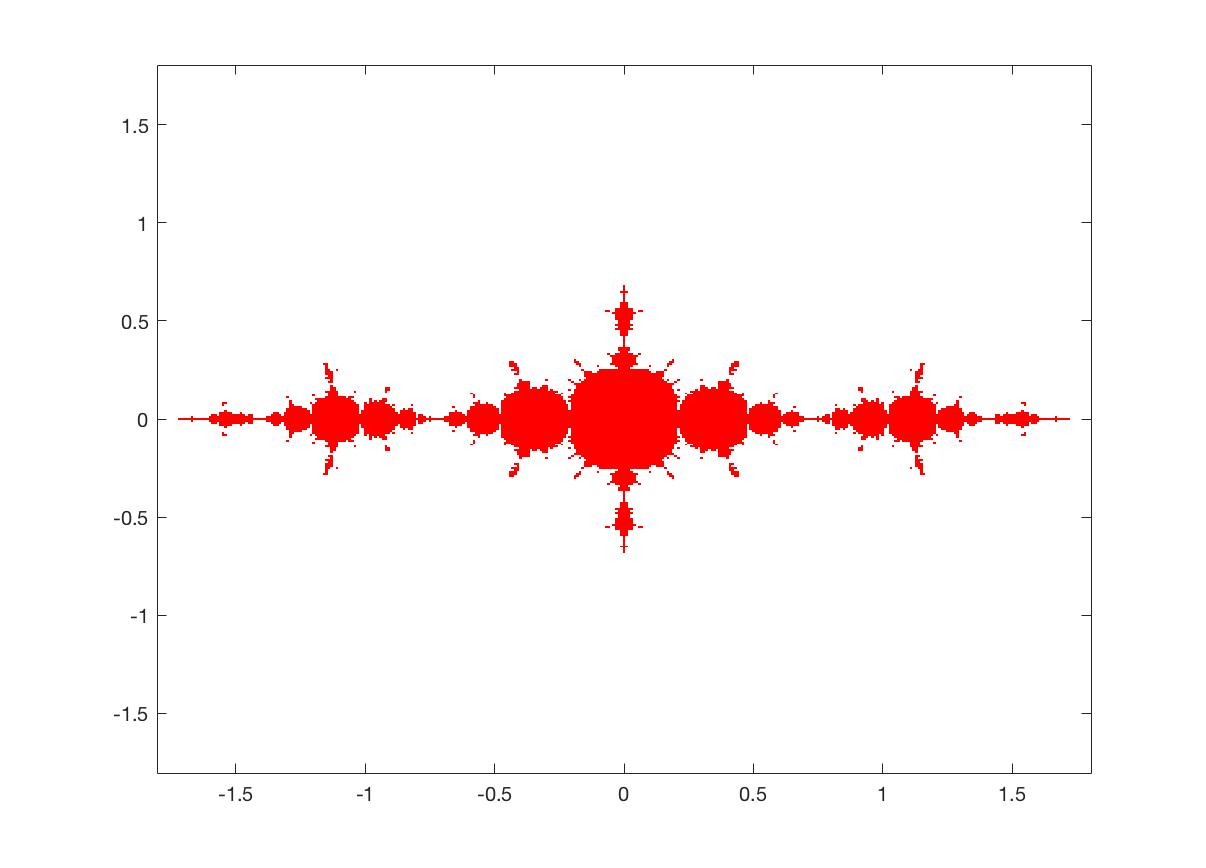
\includegraphics[width=0.7\linewidth]{Julia_Set_1}
		\caption{}
		\label{fig:juliaset1}
	\end{subfigure}
	
	\begin{subfigure}{0.5\textwidth}
		\centering
		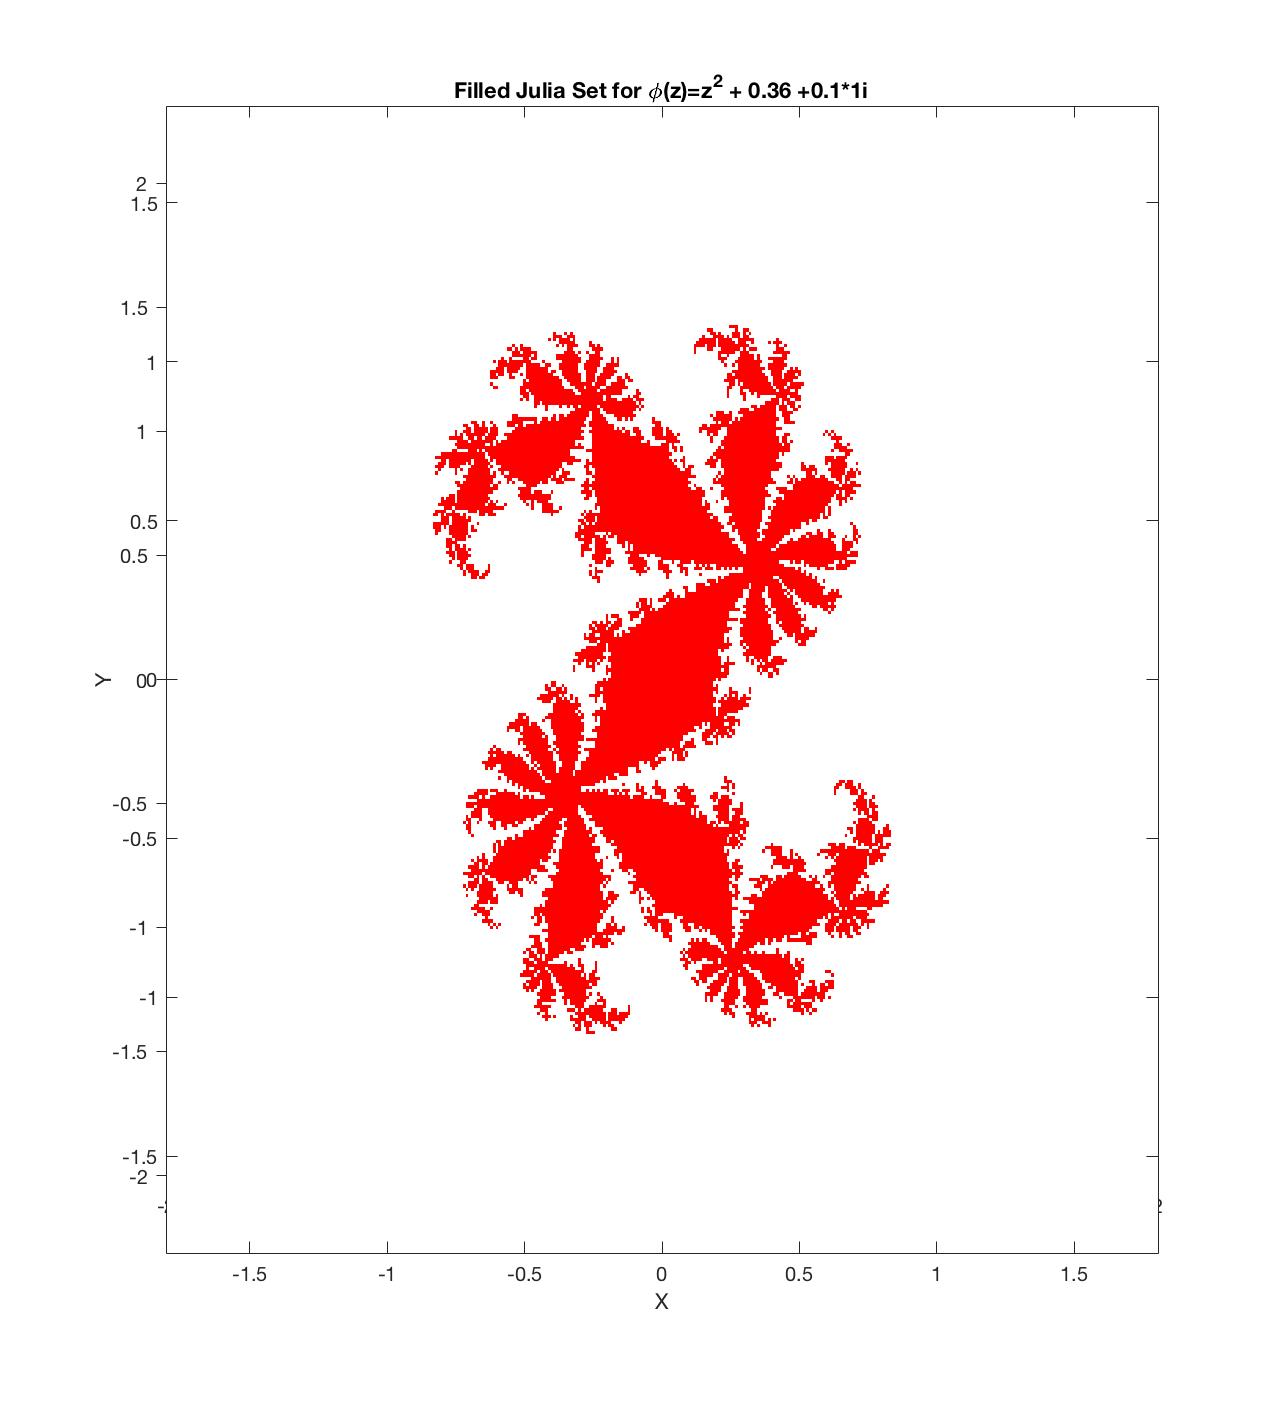
\includegraphics[width=0.7\linewidth]{JuliaSet_4}
		\caption{}
		\label{fig:juliaset4}
	\end{subfigure}
	\caption{Plots of various Julia Sets}
\end{figure}


\subsection{Boundaries of Filled Julia Sets}\label{prob3}
	We also can form the Julia set by plotting the boundary of the filled Julia sets from section \ref{prob2}. Boundary points are found by noticing that if $\phi(z)=z^2+c$, then $z= \pm \sqrt{\phi(z)-c}$. So, if $z_k = \phi(z_{k-1})$ we get that $z_k= \pm \sqrt{\phi(z_k)-c}=\pm \sqrt{z_{k+1}-c}$, which provides an iterative method to move backwards in the sequences used to generate filled Julia sets. Below is the sample code and Julia sets from \ref{prob2}.
	    \begin{verbatim}
	% plots Julia set for z^2 +c
	c= 0.36+.1*1i;   % Define the function whose fixed points we seek.
	
	phiInv= @(z) sqrt(z-c); %this is the inverse iteration of a point
	
	%these holds the real values of the points on the boundary of the filled Julia sets
	Rphi=[200^2];
	Iphi=[200^2];
	arraycount=0;
	
	for j=1:201                  % Try initial values with imaginary parts between
	y = -1+ (j-1)*.01;        %   -1 and 1
	for i=1:201                % and with real parts between
	x = -1 + (i-1)*.01;     %   -1 and 1.
	arraycount=arraycount+1; %increment the Iphi/Rphi arraycount
	zk=x+y*1i;      %set zk to the point in the [-1,1]x[-1,1] region
	kcount=0;       %counter for reverse iteration
	
	%run reverse iteration untill it reaches boundary, kick out if it
	%diverges
	while kcount < 100 && abs(zk) < 2
	n=randi(2,1);
	y=imag(zk-c);
	kcount = kcount+1;
	zk=(-1)^n*phiInv(zk);
	
	end
	%zk is now on the boundary, so set the real and imaginary arrays to its
	%value there
	if abs(zk)<2
	Rphi(arraycount)=real(zk);
	Iphi(arraycount)=imag(zk);
	end
	end
	end
	%plot the Rphi vs Iphi
	scatter(Rphi,Iphi,'.')
	pbaspect([1 1 1]);  %keep aspect ration square
	
	
	\end{verbatim}
	
	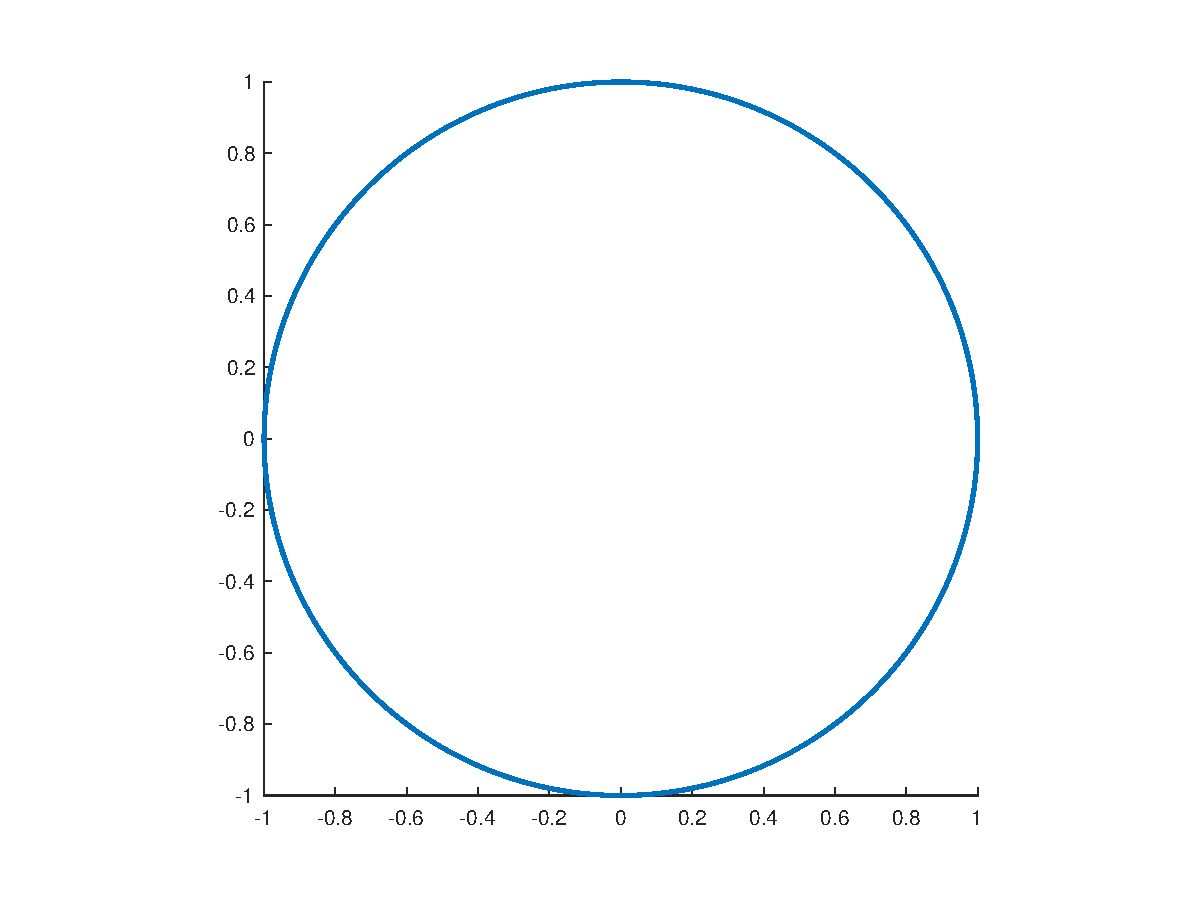
\includegraphics[width=0.49\linewidth]{juliaBound_1.eps}
	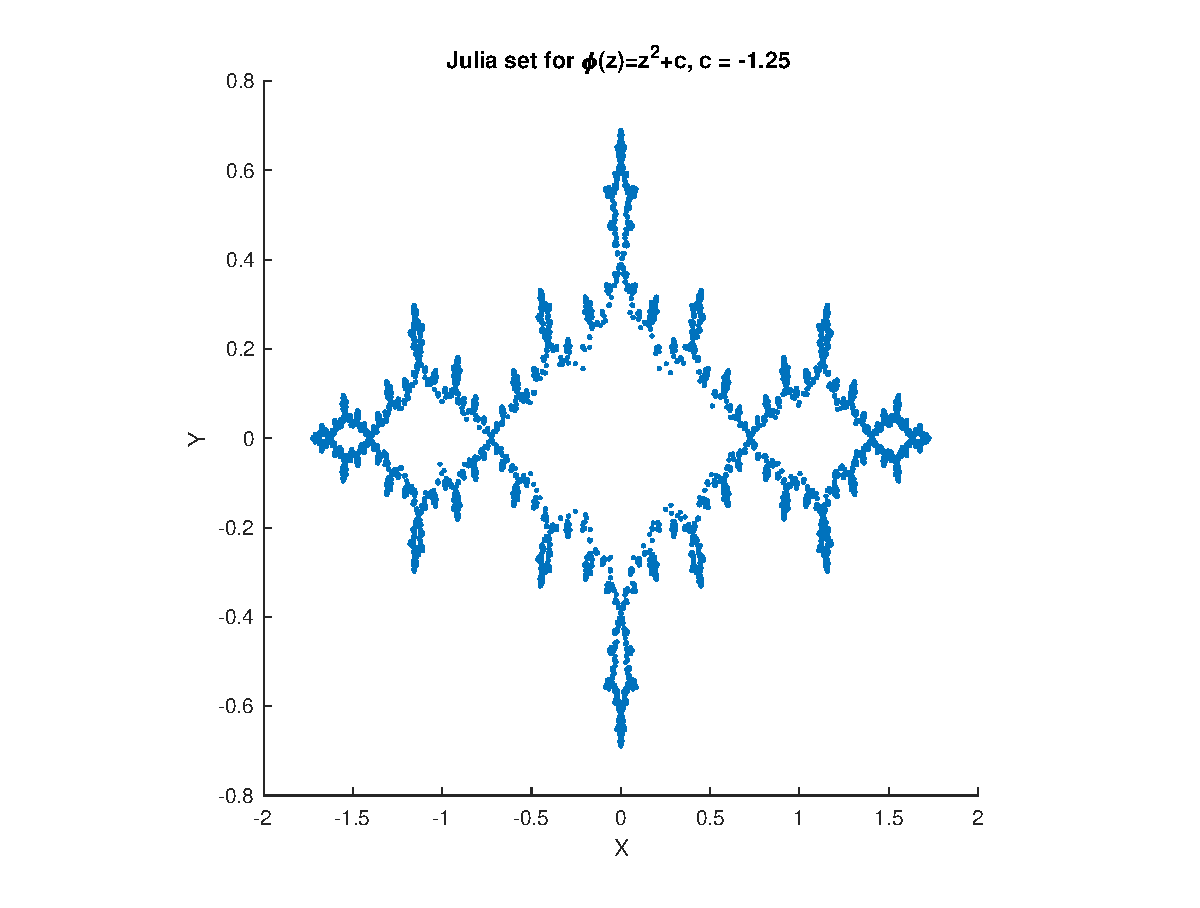
\includegraphics[width=0.49\linewidth]{juliaBound_2.eps}
	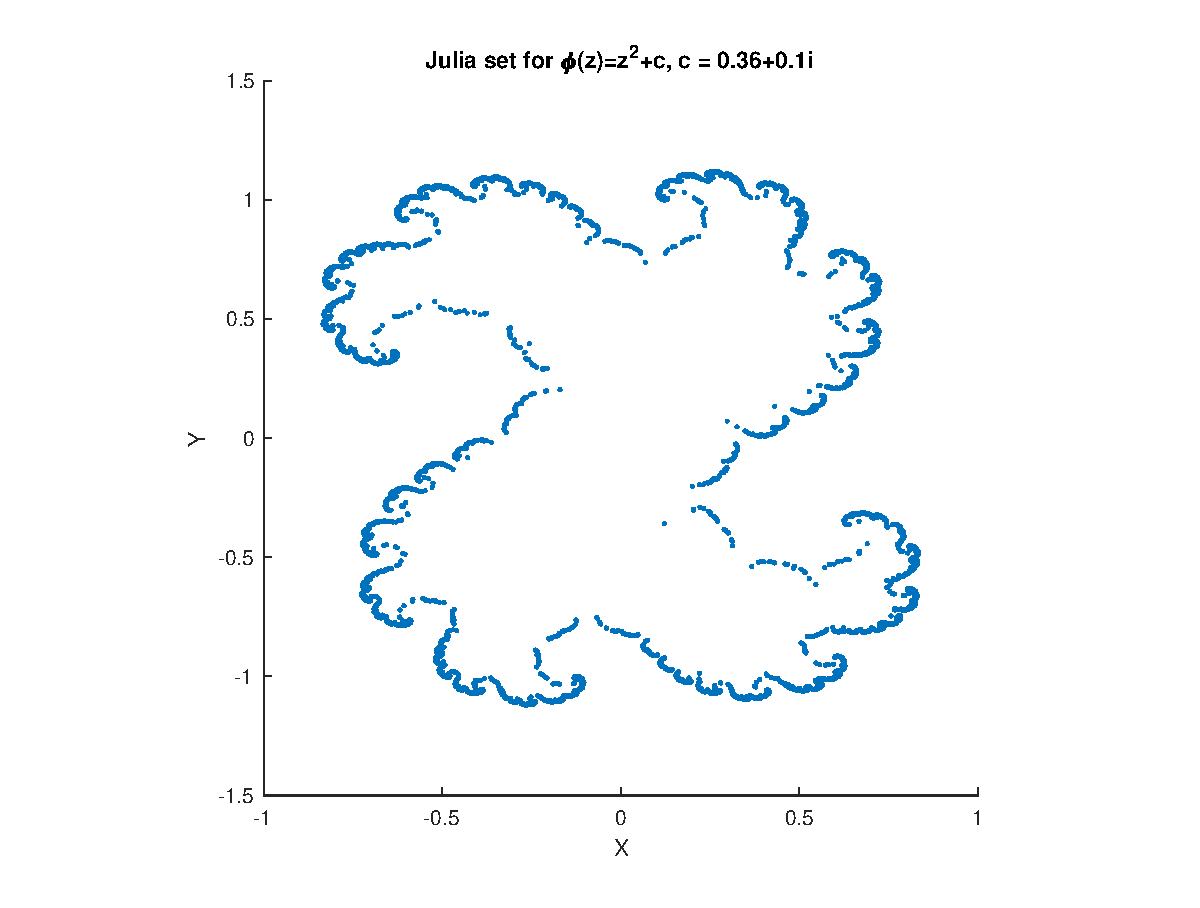
\includegraphics[width=0.49\linewidth]{juliaBound_3.eps}
	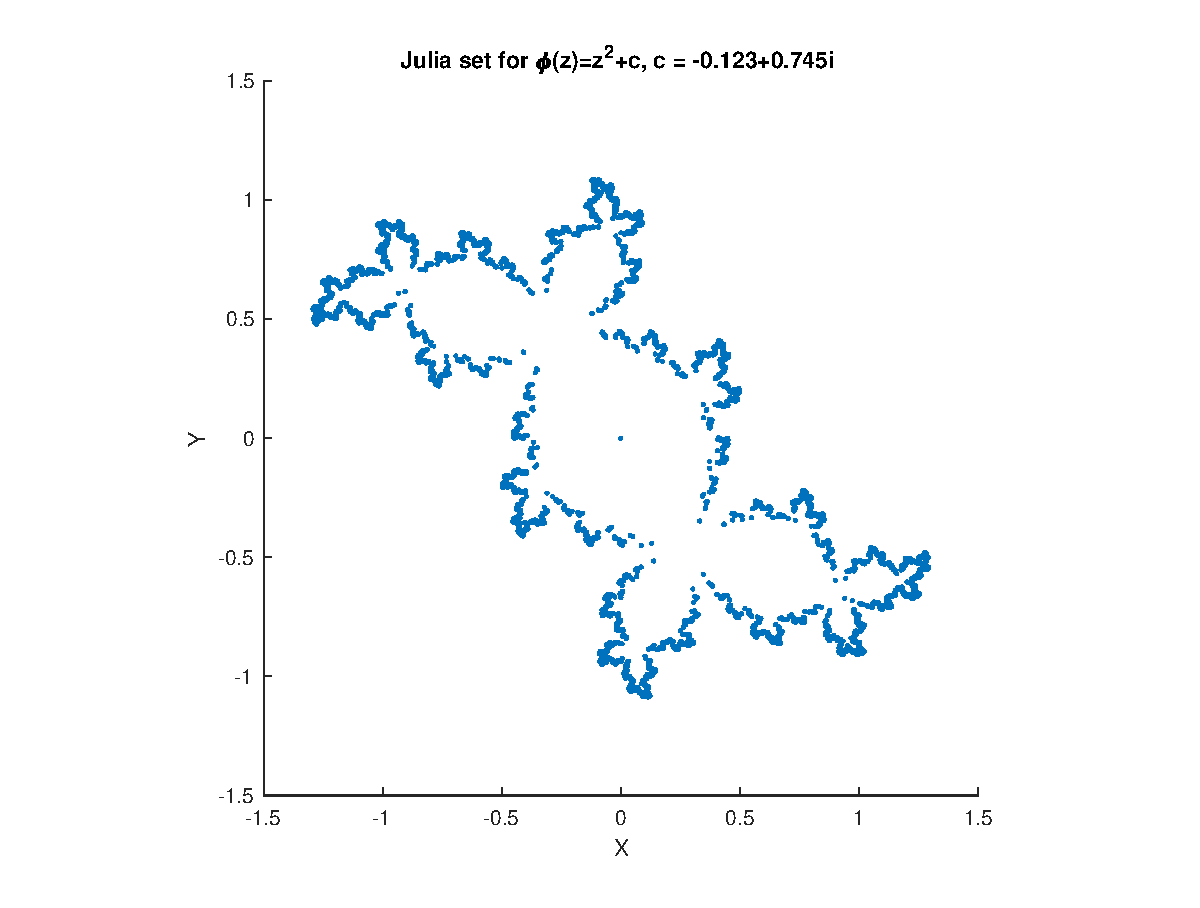
\includegraphics[width=0.49\linewidth]{juliaBound_4.eps}

\section{Computing Fractal Dimentions}

\section{Orbits}

While the filled Julia set studies whether or not the initial starting point $z_0$ will produce a bounded or converging sequence $\{z_n\}$ under $\phi$, it can be worthwhile to investigate the sequence $\{z_n\}$ itself. We do this by looking at the orbit of a particular $z_0$, where the orbit (denoted by $orb(z_0)$) is given by the set of all elements in the sequence $\{z_n\}$ generated by $\phi$. 
	
\subsection{Connectedness of the Filled Julia Set}
The complex nature of Julia Sets brings up the question of whether or not the filled Julia set is connected (in the topological sense). Surprisingly, there is a simple necessary and sufficient condition for connectedness. Julia and Fatou showed that the filled Julia set for $\phi(z)=z^s+c$ is connected if, and only if, $0$ is in the filled Julia set. Using this condidtion, we develop an algorithm that checks whether or not the $orb(0)$ for a particular $\phi$ is bounded. Boundedness implies that $0$ is in the filled Julia set for $\phi$, so the set is connected. From an algorithmic standpoint, it is difficult to determine with complete certainty that an orbit is bounded since the orbit may remain bounded for many terms and then diverge, or it might grow quickly and then cycle and remain bounded. So, our algorithm checks the first 1000 terms of $orb(0)$ and if the terms remain bounded by 100, we conclude that $orb(0)$ is bounded.    
\subsection{Coloring Divergenet Orbits}
We can also study how fast an orbit diverges. We do this by computing the sequence $z_n$ generated by $phi$. When $|z_k|>1000$ for some $k$, we assign a color to the matrix element corresponding the location of $z_k$ in the complex plane. For colors that diverge at similar points in the sequence (I.e for similar $k$ values), the color is similar. Printing this gives a good idea at how fast points near the boundary of the filled Julia set are diverging. Below is the algorithm, and a sample output for $\phi(z)=z^2+0.36+0.1\cdot i$.\\ 
   \newline
   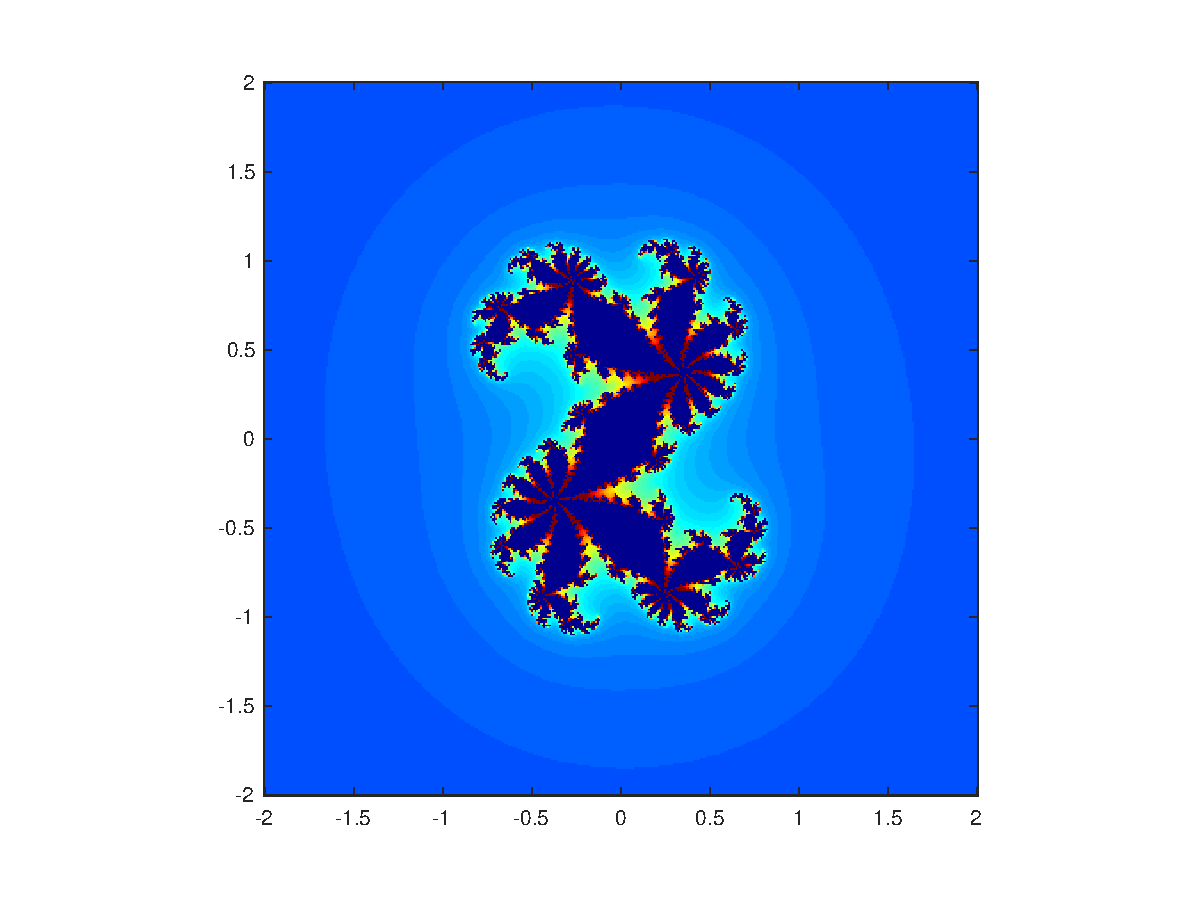
\includegraphics [width=4in]{ColorOrbit_01.eps}
   
    \begin{verbatim}
% Checks the orbits of z_0 from the region [-2,2]x[-2,2]
% under phi(z)=z^2+c

%Define the c
c=0.36+0.1*1i;

%Define the functions and fixed points.
phi = @(z) z^2 + c;
fxpt1 = (1 + sqrt(1-4*c))/2;
fxpt2 = (1 - sqrt(1-4*c))/2;

colormap jet;
M= zeros(401,401);
for j=1:401                  % Try initial values with imaginary parts between
y = -2+ (j-1)*.01;        %   -2 and 2
for i=1:401                % and with real parts between
x = -2 + (i-1)*.01;     %   -2 and 2.
z = x + 1i*y;
zk = z;

iflag1 = 0;     % iflag1 and iflag2 count the number of iterations
iflag2 = 0;     %   when a root is within 1.e-6 of a fixed point;
kcount = 0;      % kount is the total number of iterations.


while kcount < 1000 && abs(zk) < 100 && iflag1 < 5 && iflag2 < 5
kcount = kcount+1;
zk = phi(zk);           % This is the fixed point iteration.

err1 = abs(zk-fixpt1);  % Test for convergence to fixpt1.
if err1 < 1.e-6
iflag1 = iflag1 + 1;
else
iflag1 = 0;
end

err2 = abs(zk-fixpt2);  % Test for convergence to fixpt2.
if err2 < 1.e-6
iflag2 = iflag2 + 1;
else
iflag2 = 0;
end

end

if abs(zk)>100 %if the orbit diverged, fill in the color map
M(j,i)=kcount; %the color for terms that diverged with similar
%kcounts will have similar color
end
end
end

image([-2 2],[-2 2],M),  % This plots the results.
pbaspect([1 1 1]); %keeps the x/y ratio even
axis xy % prevents inverted xy axis
\end{verbatim}


\section{A Newton's Method Approach}

\section{Mandelbrot Sets}
As opposed to Julia sets which study the boundedness of the sequence $\{z_n\}$ for fixed $\phi$, we can choose to check whether the filled Julia set is connected for varying $\phi$ by changing the constant $c$ values. That is, given $c\in \C$, define $\phi(z)=z^2+c$, and check $orb(0)$ for $phi$. Studying which $c$ produces bounded zero-orbits gives the Mandelbrot set. Below is an image of the Mandelbrot set and an algorithm which computes the set. \\
 
 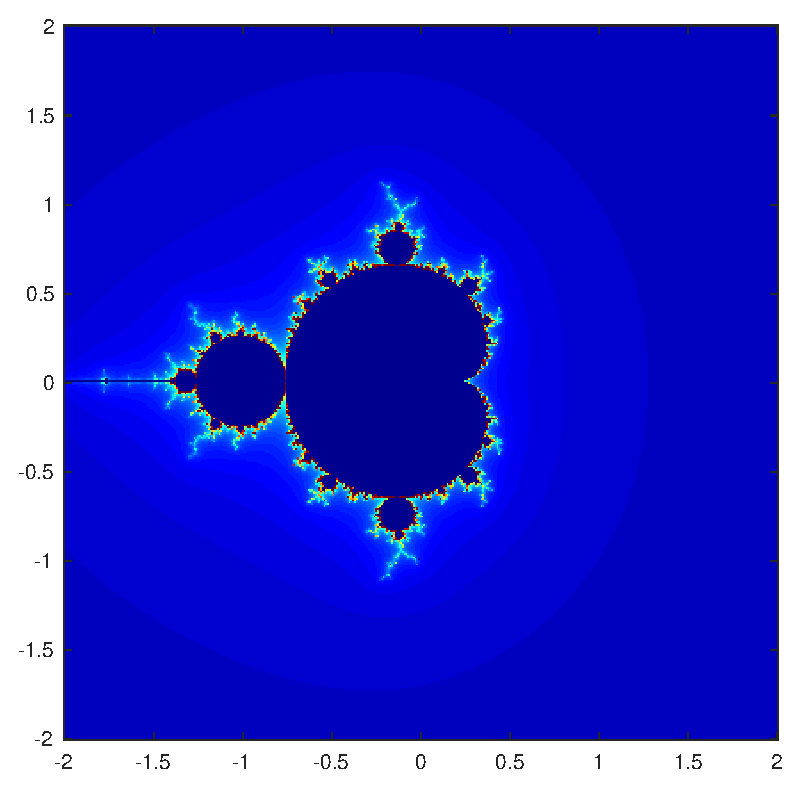
\includegraphics [width=4in]{Mandelbrot_01.eps}
 
 \begin{verbatim}
% This program generates the mandelbrot set

%Define the functions and fixed points.
phi = @(z,c) z^2 + c;
fixpt1 = @(c) (1 + sqrt(1-4*c))/2;
fixpt2 = @(c) (1 - sqrt(1-4*c))/2;
z0=0;       %madelbrot uses z0=0;
colormap jet;

M= ones(401,401);
for j=1:401                  % Try initial values with imaginary parts between
y = -2+ (j-1)*.01;        %   -2 and 2
for i=1:401                % and with real parts between
x = -2 + (i-1)*.01;     %   -2 and 2.
c = x + 1i*y;


iflag1 = 0;     % iflag1 and iflag2 count the number of iterations
iflag2 = 0;     %   when a root is within 1.e-6 of a fixed point;
kcount = 0;      % kount is the total number of iterations.
zk=z0;
%compute the orb(0) for this particular c value
while kcount < 1000 && abs(zk) < 100 && iflag1 < 10 && iflag2 < 10
kcount = kcount+1;
zk = phi(zk,c);           % This is the fixed point iteration.

err1 = abs(zk-fixpt1(c));  % Test for convergence to fixpt1.
if err1 < 1.e-6
iflag1 = iflag1 + 1;
else
iflag1 = 0;
end

err2 = abs(zk-fixpt2(c));  % Test for convergence to fixpt2.
if err2 < 1.e-6
iflag2 = iflag2 + 1;
else
iflag2 = 0;
end

end

if abs(zk)>100 %if the orbit diverged, fill in the color map
M(j,i)=kcount; %the color for terms that diverged with similar
%kcounts will have similar color
end
end
end

image([-2 2],[-2 2],M),  % This plots the results.
pbaspect([1 1 1]); %keeps the x/y ratio even
axis xy % prevents inverted xy axis
\end{verbatim}




\section{MATLAB Code} \label{code}
	
	

	
\end{document}